\chapter{Implementation and experiments}
The design of MultiChain in the previous chapter has been fully implemented.
In this chapter we test if MultiChain is correctly implemented according to the design
and we experiment the MultiChain in various scenarios.
MultiChain is experimented with to test if it can correctly create a chain tracking a download.
Next, MultiChain is experimented with tracking anonymous downloads.
Finally, MultiChain is experimented with in potential situations where a deadlock may occur
to test if it succesfully resolve these situations.

In this chapter multiple graphs are depicted.
These graphs are generated by reading every database of every node.
The blocks are depicted as nodes and the previous hash pointers are edges in the graph.
The nodes have added colouring to indicate extra meaning.
This can be seen in Figure \ref{fig:graph-example}
Green nodes are a first block in a MultiChain of a peer,
and as such have no inbound arrows.
Blue nodes are a sequential block between the same previous peers,
therefore they do not have two inbound arrows.
Red nodes are half-signed blocks,
and therefore only have one inbound and one outbound arrow.

\begin{figure}[!h]
	\centerline{\includegraphics[scale=0.6]{experimentation/example.png}}
	\caption{Example of coloring used in Figures with graphs.}
	\label{fig:graph-example}
\end{figure}

Some experiments were also run multiple times because Dispersy does not always connect to every peer.
At the start of the experiment the peers are forced to be introduced,
but this does not always succeed.
This is a problem in discoverability and has been experienced by previous work aswell~\cite{ruigrok-anonymous}.
The final version is chosen when Dispersy did connect all the peers.
We recommend that Dispersy is changed to allow a modified behaviour when experimenting
where the pool of candidates is not refreshed,
as explained in section \ref{sect:bartercast}

\section{Software engineering tests}
MultiChain is tested in several ways to verify it is correctly working
following standard software engineering practices.
These tests work similair to other tests used to test Tribler.

Tribler uses Python unit tests  to validate small components of code.
The tests can be run locally and
are automatically run on a Jenkins build server\cite{jenkins}\cite{jenkins-tribler}.
Unit tests are added to increase stability of MultiChain.
Tribler does prove to be hard to test using unit tests.
This is due to high coupling of code within Tribler.
But mocking of classes helped in testing difficult to test code.
The separate unit tests for the conversion, payload and database were the first of it types inside Tribler.
\todo{Update the table}
An overview of the coverage can be seen in Table \ref{tab:tests}

\begin{table}
\centering
\begin{tabular}{l|ll|ll}
Filename   & LOC & \%    & Conditionals & \%    \\ \hline
Community  & 187 & 86\%  & 37           & 62\%  \\
Conversion & 60  & 95\%  & 6            & 50\%  \\
Database   & 113 & 87\%  & 10           & 50\%  \\
Payload    & 89  & 100\% & 2            & 100\% \\ \hline
Total      & 672 &       & 47           &
\end{tabular}
\caption{Unit tests coverage of MultiChain.}
\label{tab:tests}
\end{table}

Next to that, Tribler uses a separated developed test runner Gumby.
Gumby can start multiple instances of Tribler and follow test scenario's.
Gumby can be used to perform system tests and experiments.
These system tests have to be manually validated.
Several scenario's have been written to validate MultiChain.
These run MultiChain either in a standalone version or integrated into the TunnelCommunity.

One of these scenario's can be found in Listing \ref{fig:exp-gumby-scenario}
In this example basic block creation is tested.
Normal situations are tested,
but also situations where the signature requests are answered late
and other requests arrive at the requesting peer at the same time.
Additionally, signature requests are controlled to not be answered at all.
During the whole test the crawler is active and scrapes the network for unknown blocks.
The notation in the scenario is the time an action has to be taken place,
the action that has to be taken, and by who if necessary.

\begin{figure}
\begin{FVerbatim}[fontsize=\small]
@0:0 set_master_member 3081a7301006072a8648ce ... 2b51
@0:0 set_community_class MultiChainNoResponseCommunity {4}
@0:0 set_community_class MultiChainDelayCommunity {5}
@0:0 set_community_class MultiChainCommunityCrawler {6}
@0:0 set_community_class {6}
@0:0 start_dispersy
@0:1 online
@0:5 reset_dispersy_statistics
@0:10 annotate start-experiment-1-peer
@0:15 introduce_candidates
@0:80 request_signature 2 {1}
@0:84 request_signature 1 {2}
@0:94 request_signature 4 {1}
@0:95 request_signature 1 {3}
@0:104 request_signature 5 {1}
@0:106 request_block 1 5 {6}
@0:110 close
@0:111 stop_dispersy
@0:112 stop
\end{FVerbatim}
    \caption{One fo the gumby test scenarios}
    \label{fig:exp-gumby-scenario}
\end{figure}

\section{Tracking download and upload amounts}
In this section we will experiment with MultiChain creating blocks and tracking download and upload amounts of peers.
We will first start with creating a simple block in an experiment.
The next experiment is to try to create a chain of blocks with mimicking a download of 10MB
and a larger download of 10GB.
Downloads are done at different download speeds and an experiment was done to test MultiChain in this environment.

\section{Single block creation}
In this experiment we try to create a block between two nodes.
This experiment validates the MultiChain to be able to correctly create a block between nodes in normal circumstances.
The experiment is locally run using gumby with all nodes running on a single computer.
Only two instances of MultiChain communities are started and between these two communities a block is created.
The logging of the both nodes is captured and recorded to verify the results of the experiment.

The output of the logging can be seen in figure \ref{fig:singleblockexperiment}.
First node 1 sends a signature request to node 2.
This message is received and a block is persisted.
The hash of the block is displayed in the output.
The block is sent back as a signature response to node 1.
The block is saved by node 1 and has the same hash as shown in the output.
So the block between node 1 and node 2 is the same and a block was succesfully created.
The output also shows behaviour of MultiChain
to correctly exclude any other execution from entering mutual exclusive code.
The lines related to the mutual exclusion are prepended by "Chain Excl".
The nodes check if it is possible to enter the mutual exclusive part and correctly acquires
and releases the mutual exclusion token.


\begin{figure}
    \begin{SaveVerbatim}{VerbCode}
OUT: 1: Requesting Signature for candidate: 2
OUT: 1: Chain Excl: signature request: False
OUT: 1: Chain Excl: acquired, sending signature request.
OUT: 1: Sending signature request.
OUT: 2: Received signature request.
OUT: 2: Chain Excl: process request: False
OUT: 2: Chain Excl: acquired to process request.
OUT: 2: Persisting sr: 2F7bTMxyJU7hZkvaBimT2bYm4bY=
OUT: 2: Chain Excl: released after processing request.
OUT: 2: Sending signature response.
OUT: 1: Signature response received. Modified: True
OUT: 1: Valid 1 signature response(s) received.
OUT: 1: Persisting sr: 2F7bTMxyJU7hZkvaBimT2bYm4bY=
OUT: 1: Chain Excl: released after signature response.
    \end{SaveVerbatim}
    \setlength{\fboxsep}{5mm}
    \fbox{\BUseVerbatim{VerbCode}}
    \caption{Output of single block creation experiment}~\label{fig:singleblockexperiment}
\end{figure}
\subsection{Chaining blocks}
The next experiment we experiment with MultiChain creating a chain of blocks between two peers.
The experiment is run using gumby with all peers running on a single computer.
We try to create 10 subsequent blocks mimicking a download of 10MB with a speed of 1000 KB/s.
Every second these amounts are indicated to have been transferred to the schedulers of every peer.
The scheduler waits for 1MB uploaded to another peer before scheduling a block.

The result of the experiment can be seen in the graph in Figure \ref{fig:chain-experiment-graph}.
In this graph it can be clearly seen that MultiChain is succesful in creating a chain of 10 blocks.

\begin{figure}[!h]
	\centerline{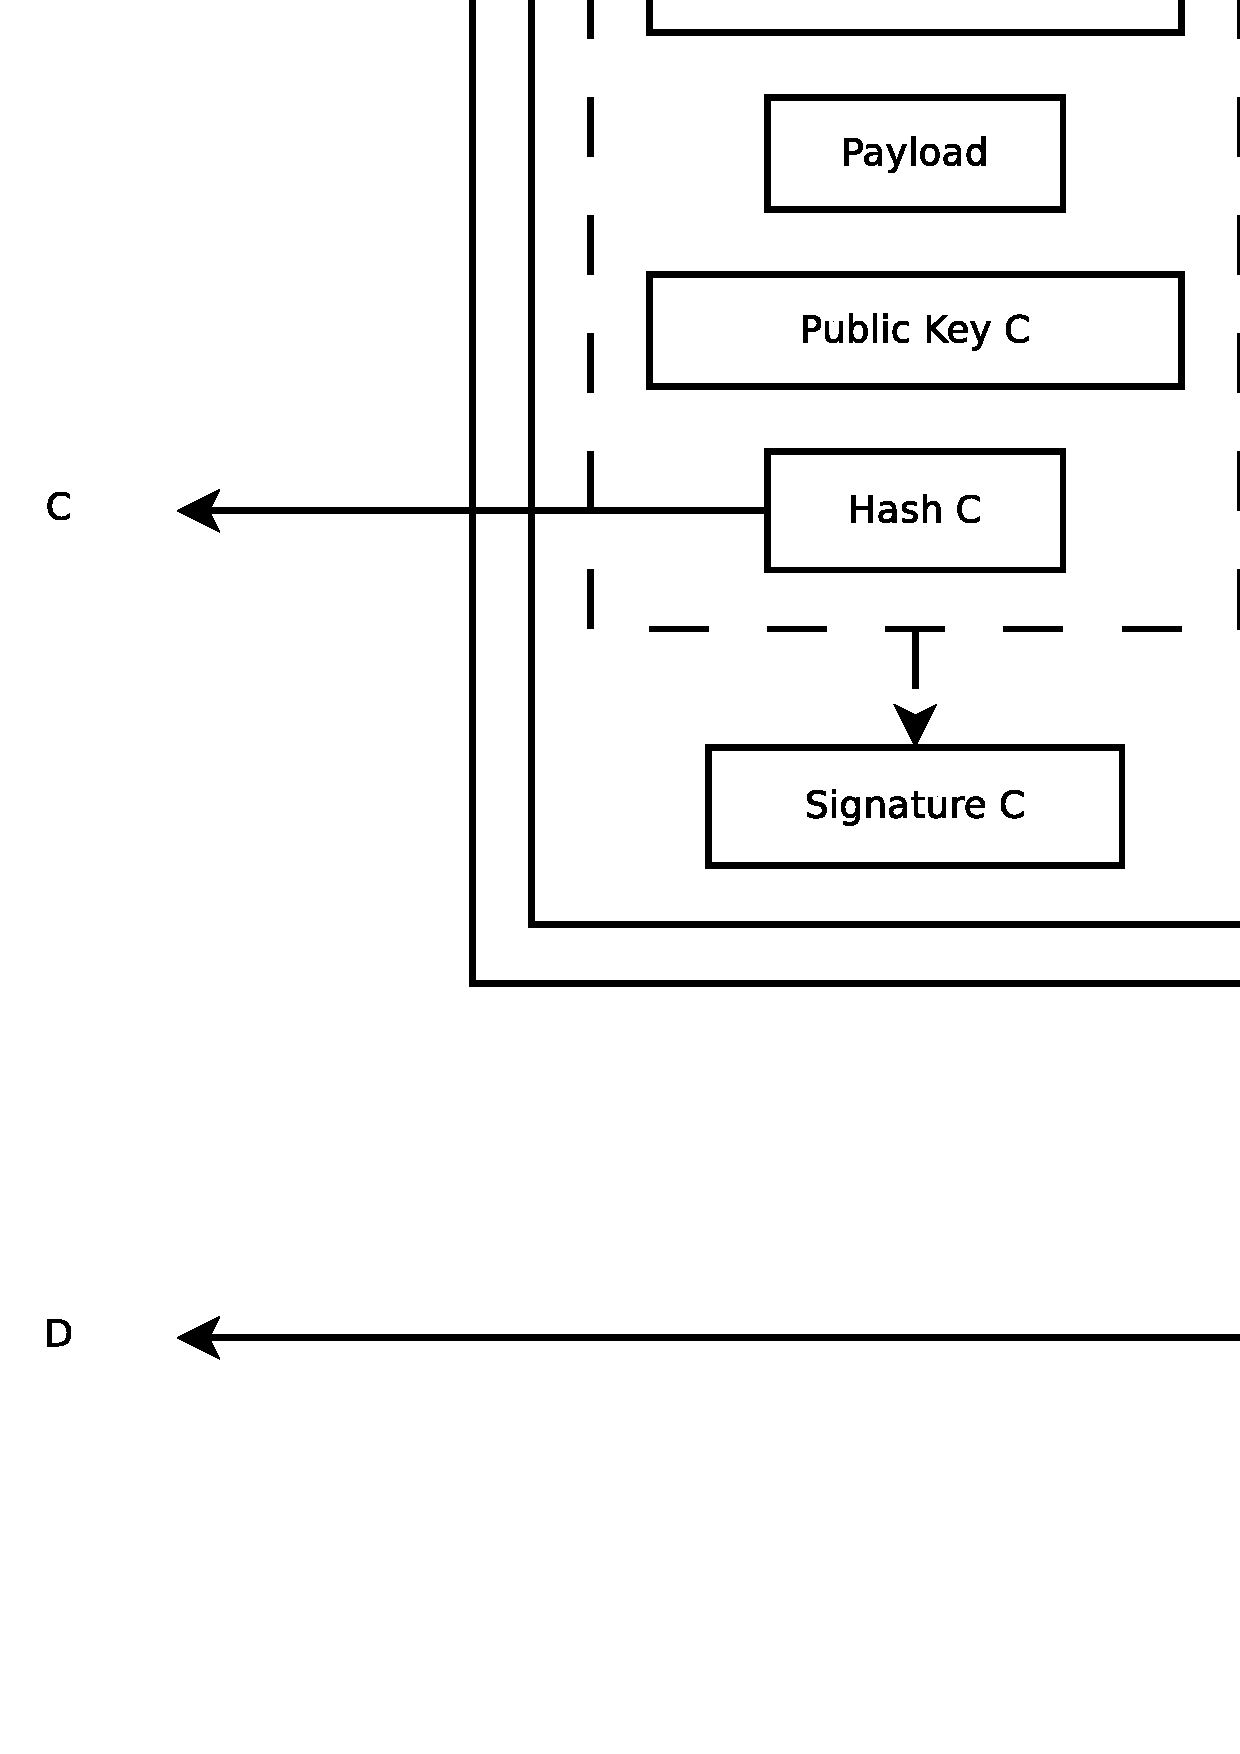
\includegraphics[scale=0.20]{experimentation/chain/chain.png}}
	\caption{MultiChain chain graph of a single download of 10 MB.}
	\label{fig:chain-experiment-graph}
\end{figure}

The amounts stored in each blocks are plotted in Figure \ref{fig:chain-experiment-amounts}.
Every datapoint is a block in the chain of a peer and is the the total amount stored in that block..
These datapoints are connected by a dotted line representing the link between these blocks.
These plots show that MultiChain correctly tracks the download of 10MB.
The slope of the figure corresponds with the speed of the download.

\begin{figure}
\centering
\subfigure[Total download amount.]{
\centerline{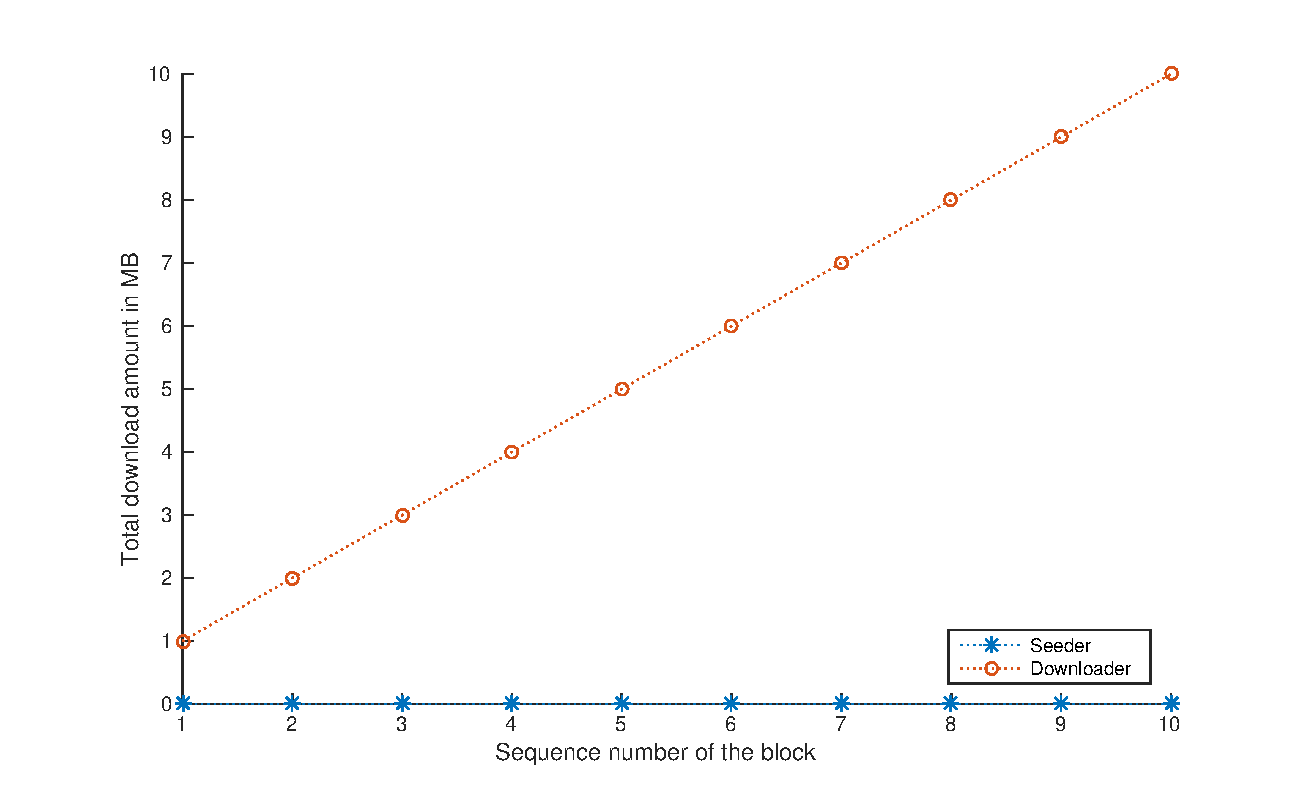
\includegraphics[scale=0.5]{experimentation/chain/chain-down.eps}}
\label{fig:chain-experiment-down}
}
\subfigure[Total upload amount.]{
\centerline{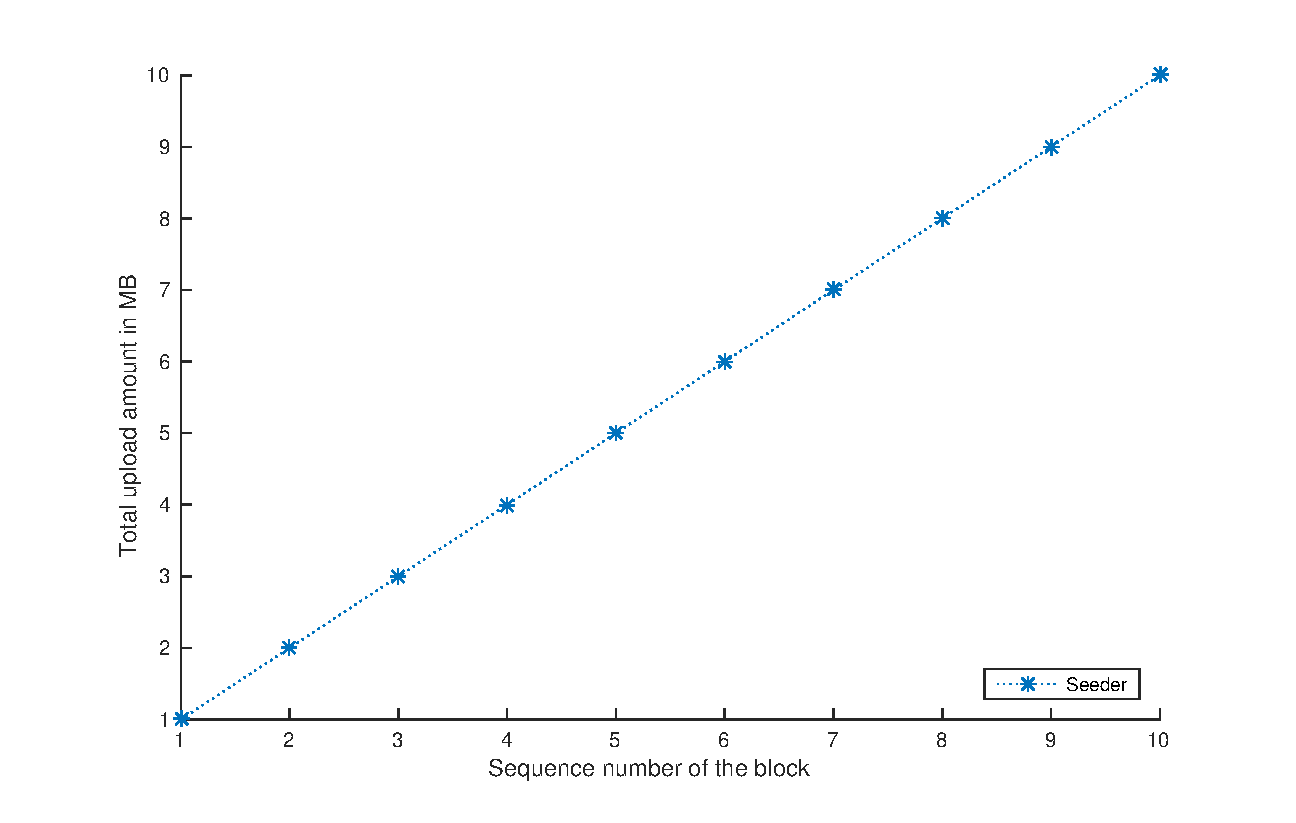
\includegraphics[scale=0.5]{experimentation/chain/chain-up.eps}}
\label{fig:chain-experiment-up}
}
\caption{Download and upload amounts when creating a chain of 10 blocks.}
\label{fig:chain-experiment-amounts}
\end{figure}

\subsection{Tracking downloads with different speeds}
In this experiment we measure if MultiChain can correctly track the upload and download amounts
between two peers with different speeds.
In the scenario a file of 100 MB is downloaded at different speeds,
respectively 500 KB/s, 750 KB/s, 1000 KB/s, 1250 KB/s, 2000 KB/s, and 3000 KB/s.
The maximum speed of anonymous download was measured in experiments to be 1150 KB/s\cite{ruigrok-anonymous}.
The scheduler waits for 1MB uploaded to another peer before scheduling a block.
The upload and download of the file is done by different pairs of seeders and leechers.
Every second these amounts are indicated to have been transferred to the schedulers of every peer.

\begin{figure}
\centering
\subfigure[Total download amount.]{
\centerline{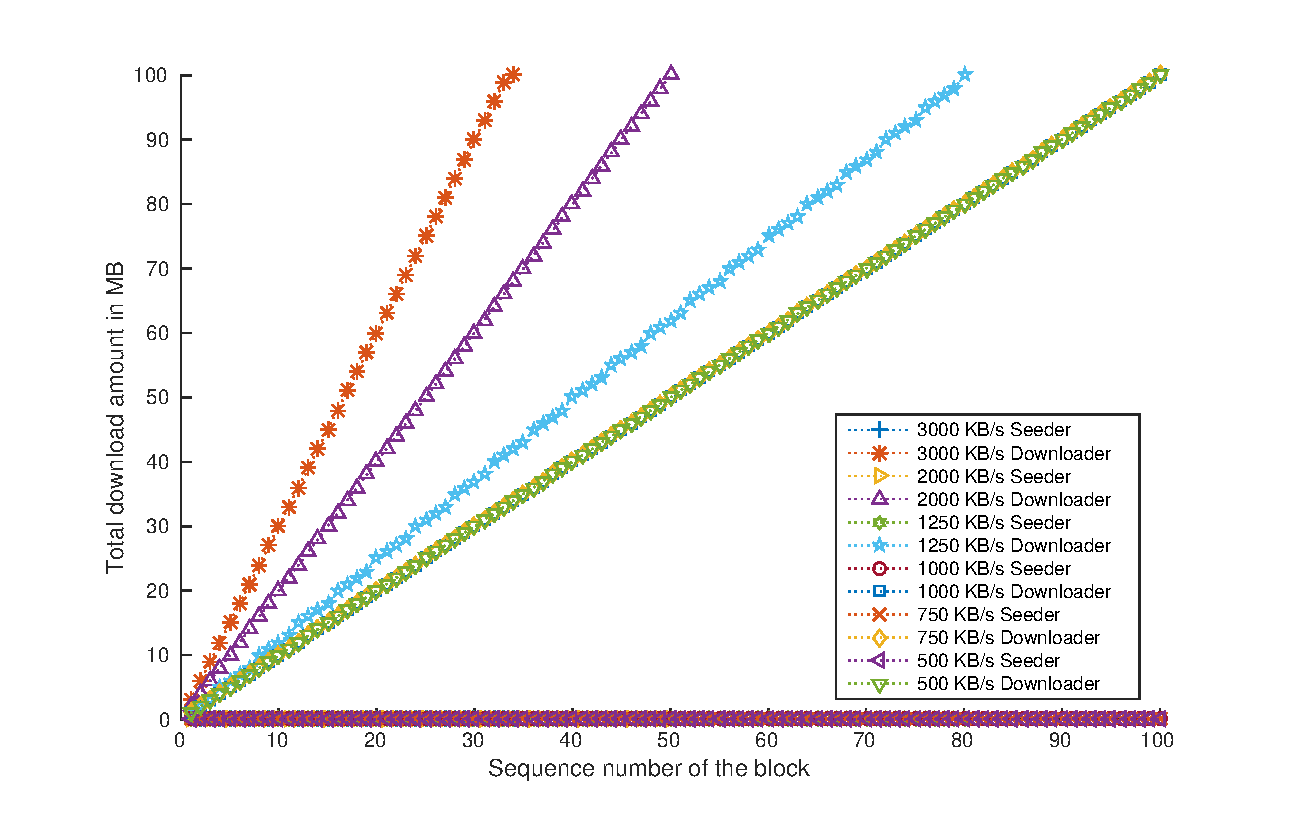
\includegraphics[scale=0.5]{experimentation/speeds/synthetic-simple-down.eps}}
\label{fig:synthetic-simple-down}
}
\subfigure[Total upload amount.]{
\centerline{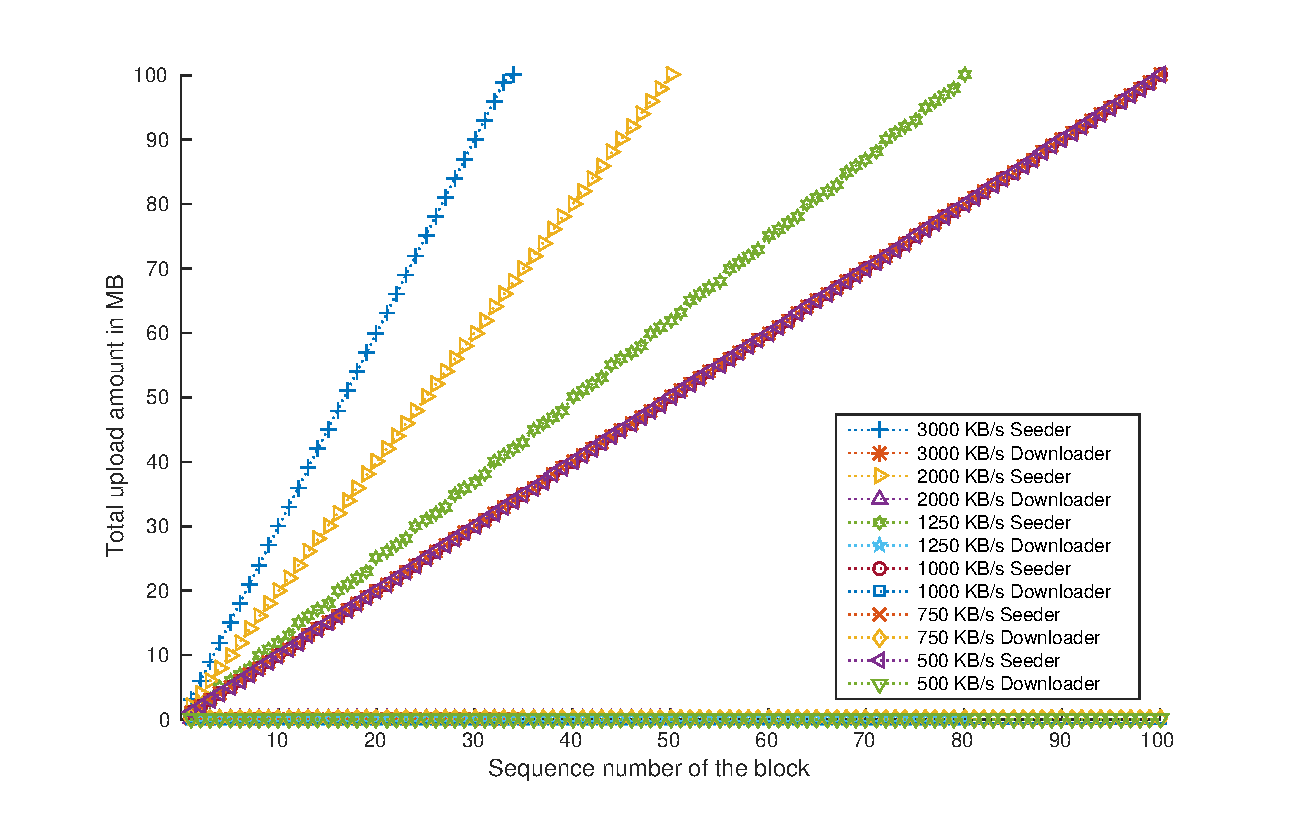
\includegraphics[scale=0.5]{experimentation/speeds/synthetic-simple-up.eps}}
\label{fig:synthetic-simple-up}
}
\caption{Download and upload amounts when tracking downloads at different speeds.}
\label{fig:synthetic-simple-amounts}
\end{figure}

The total download and upload amounts of every peer is plotted in Figure \ref{fig:synthetic-simple-amounts}.
These amounts are plotted in the same way as the previous experiment.
The plots show that MultiChain is able to correctly track the download and upload amounts without a problem.
There are no hitches in the figures and the amounts go up in fixed increments corresponding to the different speeds.
This means that MultiChain is fast enough to correctly track the amounts.

The download speeds below the threshold of 1000 MB of the scheduler
are not distinguishable from the download at the threshold speed.
This is because the scheduler waits until the threshold is reached before initiating the block.
The amount is tracked in the same amount of blocks,
but the total time of the experiment is longer for these experiments.
If the speed goes above the threshold, then this is reflected in the figure.

The graph in Figure \ref{fig:synthetic-simple-graph} shows the graph of the blocks created by the experiment.
The graph is disconnected, because the different pairs of seeders and leechers did not interact with each other.
So no block that would connect their chains is created,
This leaves the graph disconnected.

\begin{figure}
	\centerline{\includegraphics[scale=0.06]{experimentation/speeds/synthetic.png}}
	\caption{Disconnected chain graph of tracking downloads at different speeds.}
	\label{fig:synthetic-simple-graph}
\end{figure}

This experiment was run several times before the final version in this report was run.
Earlier versions of the experiment resulted in two bugfix and two improvements:
the ability of the scheduler to create a block at the end of a download.

\section{Tracking anonymous data transfer}
In this section we will experiment with MultiChain tracking anonymous data transfer.
Anonymous data transfer is a more complicated environment,
where multiple peers work together to transfer data from the seeder to the leecher.
We experiment in a synthetic environment and in environment using real anonymous downloads between peers.

\subsection{Synthetic anonymous download}
In an anonymous download scenario the data is downloaded through multiple hops.
A seeder uploads data to the first hop.
This hop relays the data to the second hop.
The second hop sends the data to its destination at the leecher.
This can be seen as sequence of peers and is illustrated in Figure \ref{fig:seeder-hops-leecher}.
More hops can be added to better safegaurd the anonymity of the download.

\begin{figure}
	\centerline{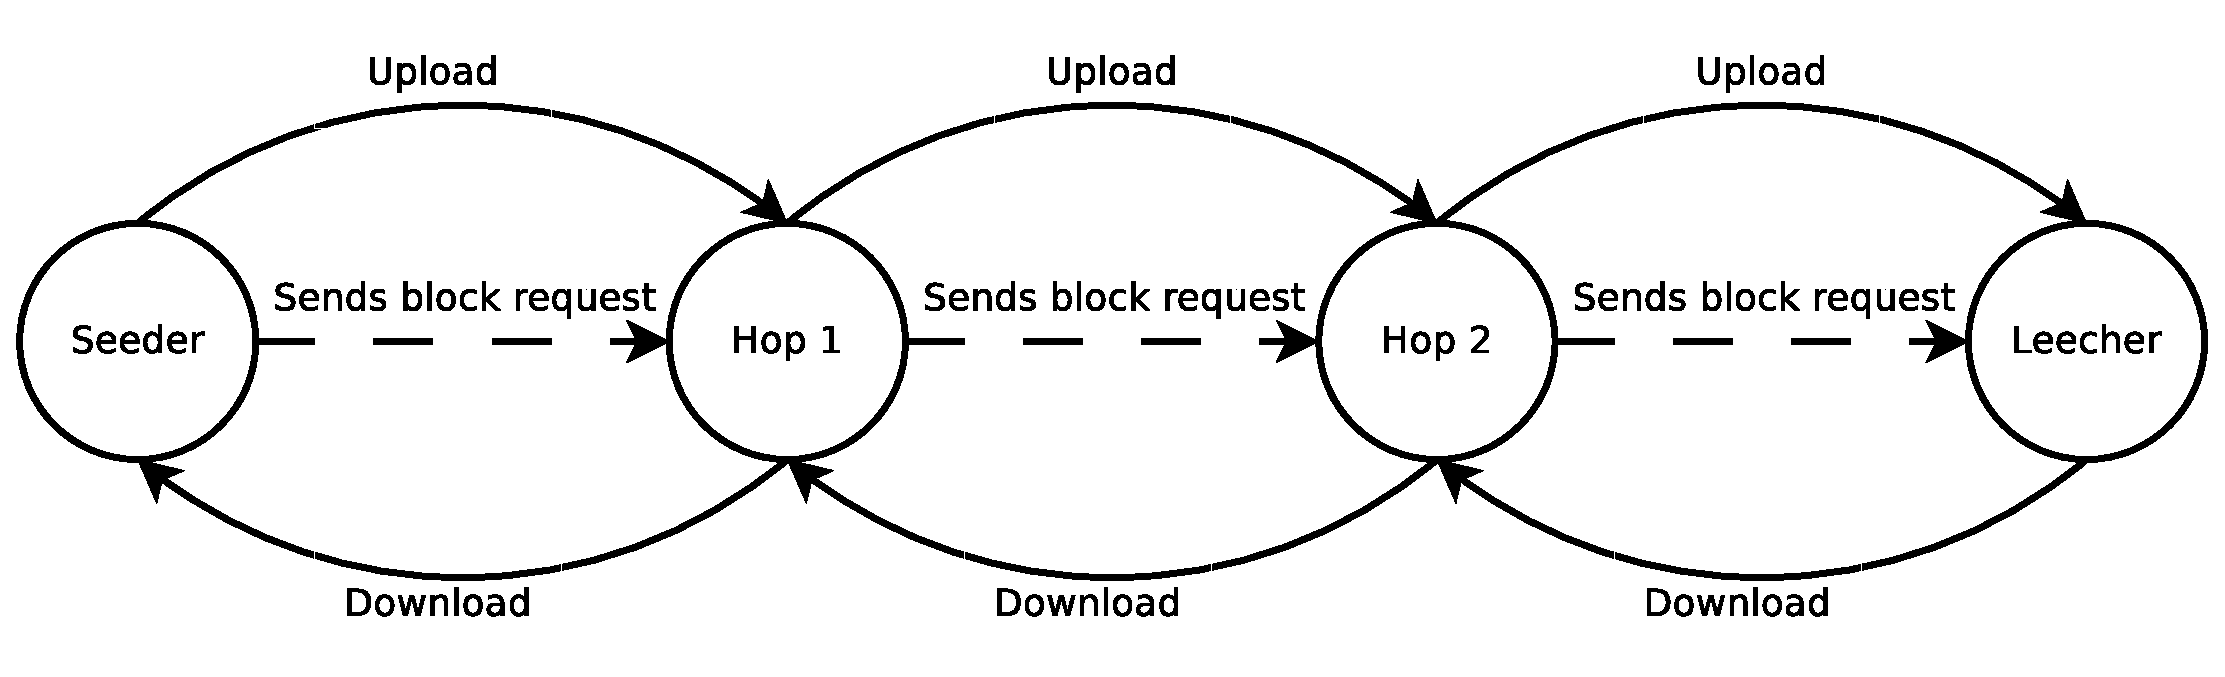
\includegraphics[scale=0.3]{experimentation/anonymous/seeder-hops-leecher.eps}}
	\caption{Block creation in an anonymous download.}
	\label{fig:seeder-hops-leecher}
\end{figure}

The total download and upload amount is plotted, in the same way as the previous experiment,
in Figure \ref{fig:synthetic-anonymous-amounts}.
The slopes of the figures are not representative for the upload and download speeds of the peers.
This is because the x-axis represents the sequence-number of the block and not time.
The hops create blocks that can be categorized in two types:
a download validating block and an upload validating block.
The download validating block only contains information about how much the hop has downloaded
and is initiated by the peer in front of the peer in the sequence.
An upload validating block is initiated by the peer itself with the peer next in the sequence.
The seeder only has upload validating blocks and as such has half the amount of blocks.
The downloader has viceversa only download validating blocks.
The slope of his figure is much steeper as a result.

In the plot a discontinuity can be found at 92\% of the download in the figures of the seeder and the first hop.
This is the result of the first hop sending a signature request to the second hop.
The second hop was not able to process this request,
because it was already working on creating another block.
The second hop drop this request.
The first hop will still wait on the second hop to process its request until it will timeout.
In turn, the seeder sent a request to the first hop that will timeout,
because the first hop is not able to process this request aswell.
During the timeouts of the seeder and the first hop,
the second hop continues to validates its own upload amounts.
No blocks are created that validate his download amount,
so the slope becomes steeper during that time and the download amount remains level.
The timeouted peers create no blocks.
When the timeouts expires, the system returns to function as normal.
In section \ref{sect:deadlock-exp} we further experiment with the timeouts in the system.

\begin{figure}
\centering
\subfigure[Total download amount.]{
\centerline{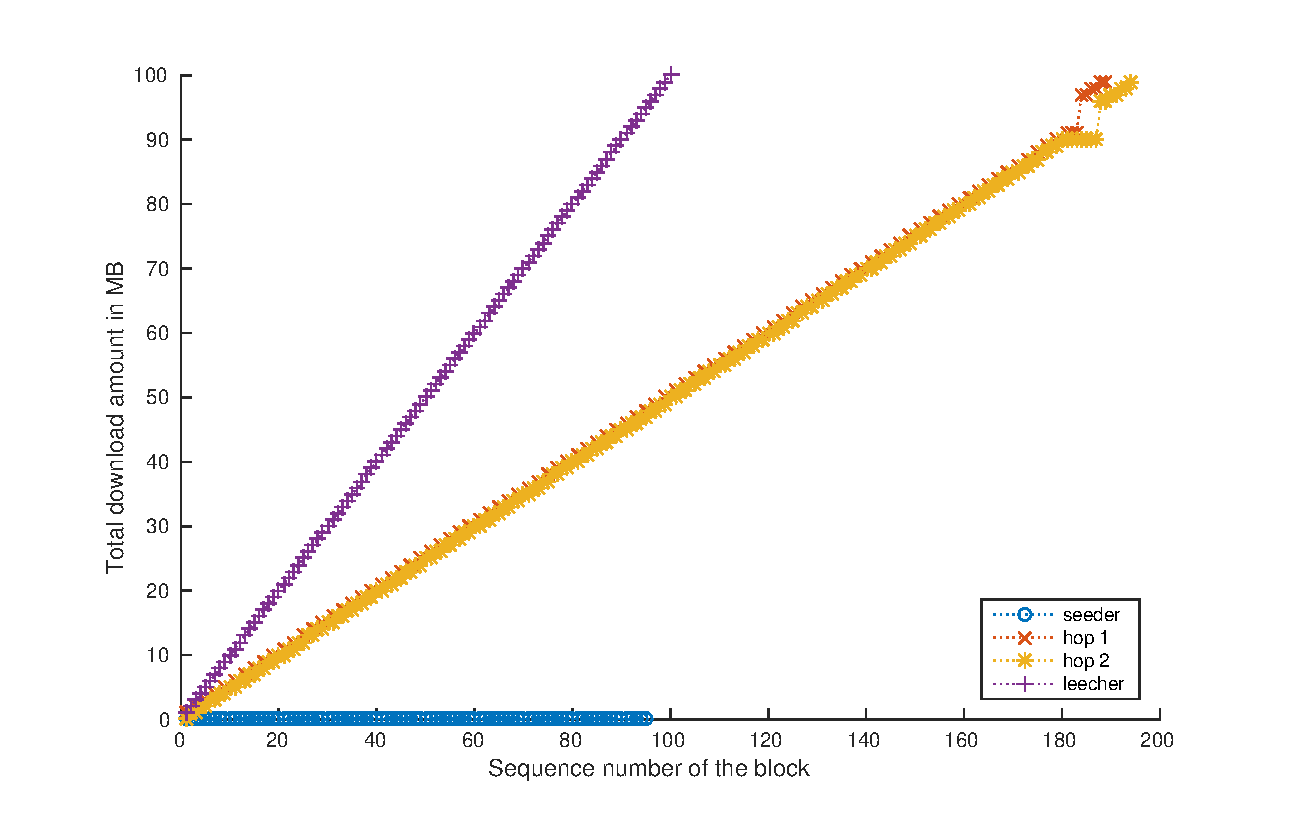
\includegraphics[scale=0.5]{experimentation/anonymous/synthetic-anonymous-down.eps}}
\label{fig:synthetic-anonymous-down}
}
\subfigure[Total upload amount.]{
\centerline{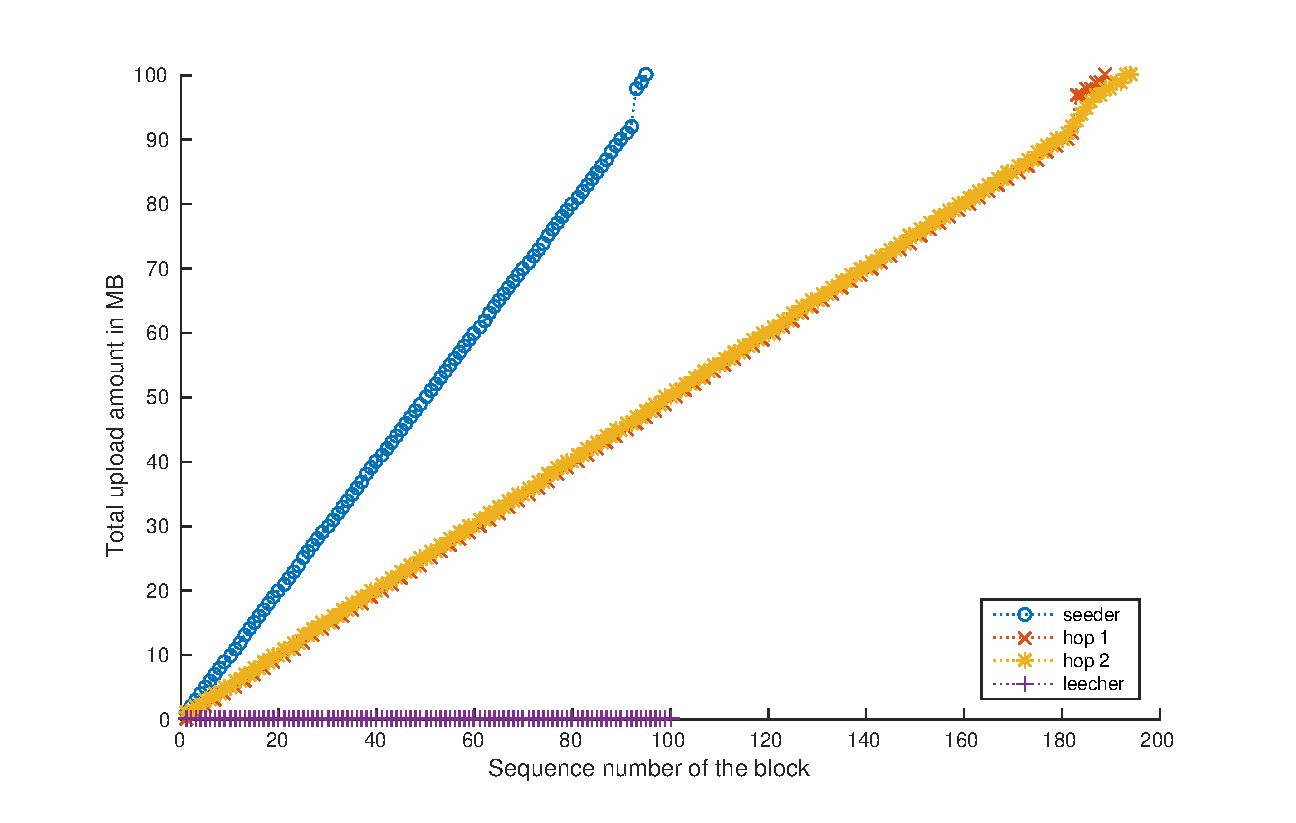
\includegraphics[scale=0.5]{experimentation/anonymous/synthetic-anonymous-up.eps}}
\label{fig:synthetic-anonymous-up}
}
\caption{Download and upload amounts during the anonymous download experiment.}
\label{fig:synthetic-anonymous-amounts}
\end{figure}

The seeder and leecher both only interact with one hop.
These hops furthermore only interact with each other.
This can be clearly seen in a part of the graph magnified in Figure \ref{fig:synthetic-anonymous-graph-magnified}.
The middle nodes represent the interaction between the hops.
The outer nodes are interactions between the seeder and the first hop and between the second hop and leecher.
The blocks are created alternating resulting in the graph pictured.

\begin{figure}
\centering
\subfigure[Partial example of expected MultiChain graph.]{
\centerline{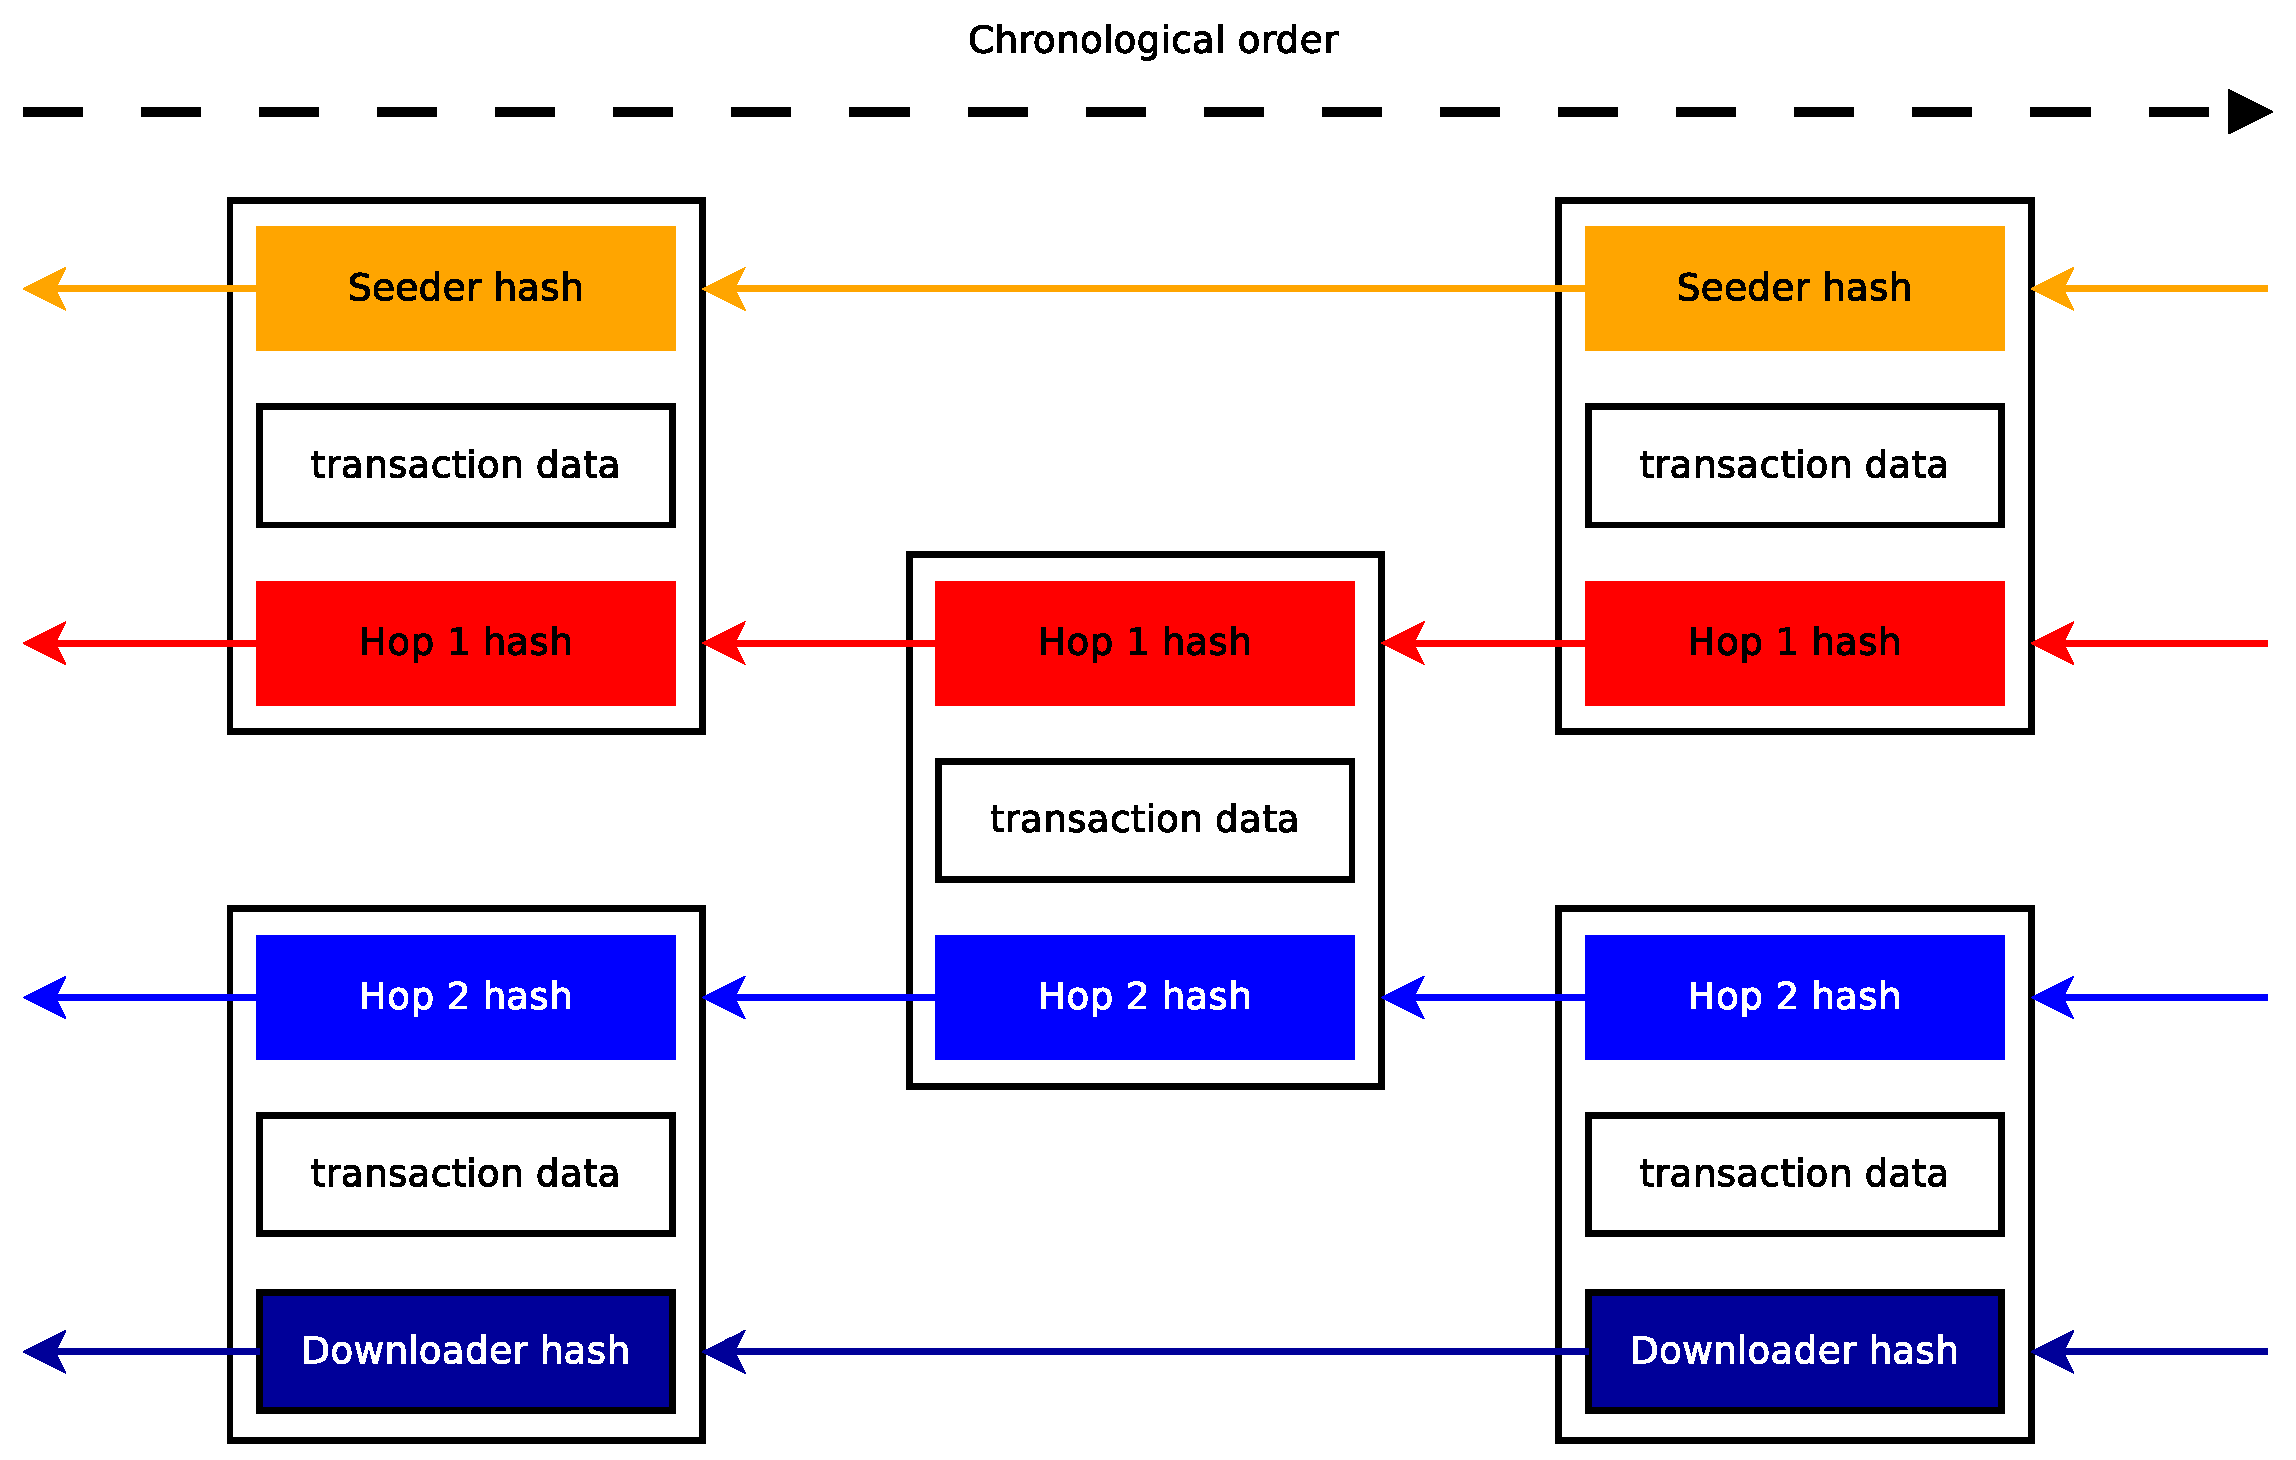
\includegraphics[scale=0.35]{experimentation/anonymous/graph-example.eps}}
\label{fig:synthetic-anonymous-graph-example}
}
\subfigure[Zoom of the actual intertwining in the MultiChain graph made with Gephi.]{
\centerline{\includegraphics[scale=0.2]{experimentation/anonymous/anonymous-magnified.png}}
\label{fig:synthetic-anonymous-graph-magnified}
}
\caption{Intertwining of the seeder and hop 1, hop1 and hop 2, and hop 2 and the downloader.}
\label{fig:synthetic-anonymous-intertwining}
\end{figure}

In the graph the timeout period can be seen clearly in Figure \ref{fig:synthetic-anonymous-timeout}.
The two half-signed block can be seen in red.
The block with a reference coming from the outer block is the half-signed block belonging to the seeder.
The strain of blue nodes are the blocks created between the second hop and the leecher.
The red inner block is referenced by the first block created between the first hop and second hop after the timeout.

\begin{figure}
	\centerline{\includegraphics[scale=0.1]{experimentation/anonymous/anonymous-timeout.png}}
	\caption{Zoom of the timeout of the seeder and hop 1, while hop 2 and the leecher continues.}
	\label{fig:synthetic-anonymous-timeout}
\end{figure}




\subsection{Integrated anonymous download}
An substantial effort was made to integrated the tunnel community and hidden services community with the MultiChain community.
These communities work together to provide functionality to transfer data anonymously.
The tunnel community reports data transferred between peers and the MultiChain community add these amounts to the chain.
They are already integrated with BarterCast.
The method of integration of BarterCast was used to try to integrated MultiChain aswell.
Setting up the Gumby environment to run all communities took also considerable time.

Experiments were conducted where an 100 MB file is transferred by the actual anonymity communities,
while MultiChain transcribes the transfer amounts in the MultiChain.
The amount of hops is varied between 0 and 2.
The result of these experiments show that the integration was not done properly.
There are two problems that were identified using the results of the experiments.

When the experiment is conducted without any hops,
the integration does not report any data transferred between the peers.
As such the scheduler never sees a reason to schedule a signature request.
The whole MultiChain community is never active.
The connection between the seeder and the first hop,
or the downloader, directly is not reported to the scheduler.

Secondly, there is a problem in the data that is reported by the data that is sent by hops.
Too much data is reported and it is unclear where this data originates from.
The overhead measures twice the actual download size.
The results can be seen in Figure \ref{fig:integrated-anonymous-amounts}.

\begin{figure}
\centering
\subfigure[Total download amount.]{
\centerline{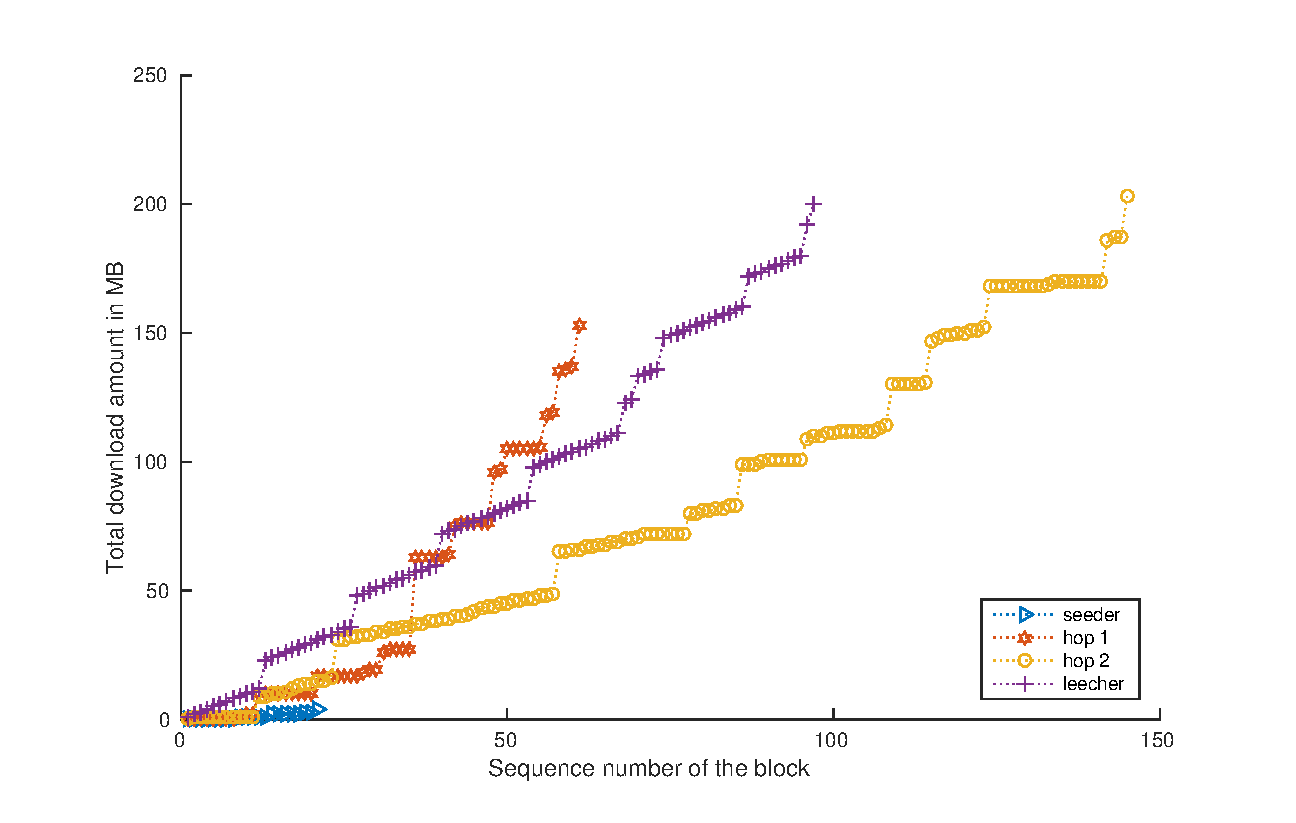
\includegraphics[scale=0.5]{experimentation/anonymous-integrated/integrated-anonymous-down.eps}}
\label{fig:integrated-anonymous-down}
}
\subfigure[Total upload amount.]{
\centerline{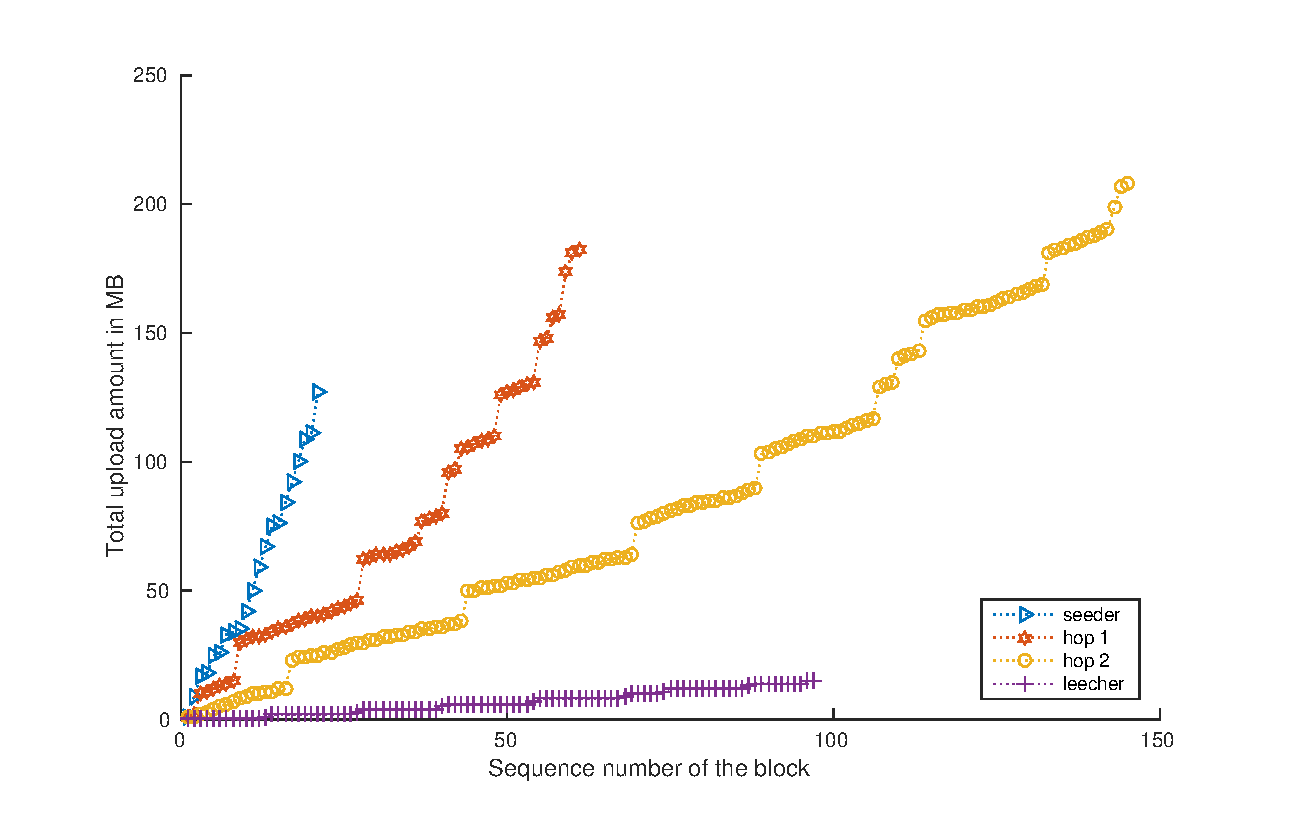
\includegraphics[scale=0.5]{experimentation/anonymous-integrated/integrated-anonymous-up.eps}}
\label{fig:integrated-anonymous-up}
}
\caption{Download and upload amounts during the integrated anonymous download experiment.}
\label{fig:integrated-anonymous-amounts}
\end{figure}

\section{Deadlock recovery}
\label{exp:deadlock}
MultiChain can run during normal operation into a situation
where two peers are both waiting on each other.
This could resulting in a deadlock.
This situation was encountered during experimentation
and the experiment shows MultiChain correctly recovering from this situation.

In the experiment a 100 megabyte file was downloaded anonymously with 2 hops.
Anonymously downloading is decribed more in the thesis report of R. Ruigrok\cite{ruigrok-anonymous}.
There are 2 Triblers instances with exit functionality and 18 instances without exit functionality.
All instances are run locally on one machine.
The instances are run in parallel,
so the fact that all instances are run on a single machine does not cause the deadlock to occur.
There is no packetloss in this experiment.

The corresponding graph of all the MultiChains of the experiment can be seen in Figure \ref{fig:deadlock-double}.
In this graph the blocks are depicted as nodes and the previous hash pointers are edges in the graph.
The nodes have added colouring to indicate extra meaning.
Green nodes are a first block in a MultiChain of a peer.
Blue nodes are a sequential block between the same previous peers.
Red nodes are half-signed blocks.

The potential scenario of two peers both waiting can be seen multiple times in the graph and are encircled.
The scenario generates a half-signed block at both peers.
Usually the peers continue collaboration and this continuation of a sequence can be seen in subsequent blocks.
In the graph a more complicated scenario can also be seen where multiple peers timeout between each other.

\begin{figure}
	\centerline{\includegraphics[scale=0.0375]{experimentation/deadlock/deadlock.png}}
	\caption{Potential deadlocks in MultiChain.}
	\label{fig:deadlock-double}
\end{figure}


\todo{Move to design}
When MultiChain has a pending signature request,
then it itself will not respond to incoming signature requests from other peers.
These peers themselves will also not respond, because they are not responding to requests for the same reason.
During seeding the seeder will mostly initiate signature requests to the downloader,
but the downloader will have some signature requests for metadata that he sents to the seeder.
These signature requests can be sent in such away that both sent the request before the other receives it.
Both peers are now waiting for the other to respond to the signature request and
will not answer the other resulting in a potential deadlock.
This deadlock can occur between two peers,
but can be expanded into a multiple of peers where each peer waits for another peer in a cycle.

MultiChain prevents this deadlock to occur
by allowing a transaction to fail as explained in section \ref{des:halfsigned}.
If MultiChain gets into this potential deadlock one of the peers will eventually time out of their own signature request
and process the incoming request.
The deadlock is recovered and both peers can continue operation.


